%%%%%%%%%%%%%%%%%%%%%%%%%%%%%%%%%%%%%%%%%%%%%%%%%%%%%%%%%%%%%%%%%%%%%%%%%
%           Capítulo 2: MARCO TEÓRICO - REVISIÓN DE LITERATURA
%%%%%%%%%%%%%%%%%%%%%%%%%%%%%%%%%%%%%%%%%%%%%%%%%%%%%%%%%%%%%%%%%%%%%%%%%
\chapter{Sistemas Hamiltonianos de dos dimensiones}
Para llegar al análisis de los sistemas de nuestro interés mediante el método de parametrización, es fundamental conocer algunos conceptos sobre la dinámica, así como del análisis numérico del mismo. En este capítulo se hace una breve descripción de los teoremas y definiciones que nos ayudarán a entender el método. Las siguientes secciones no son la manera más formal de introducir al lector a cada uno de los temas expuestos. Sin embargo proporcionan una visión puntual de lo indispensable. 

\section{Sistemas dinámicos}
Cuando uno habla sobre sistemas dinámicos, lo que le viene a la mente es alguna relación que describe el comportamiento temporal de un sistema físico. Ya sea el movimiento de péndulos o de cargas, nos interesa saber más acerca de las características de su comportamiento. 
En el estudio de los mismos se hace una clasificación en términos de sus propiedades vistas en el espacio fase o por la forma del sistema. Hay sistemas dinámicos \textit{discretos} y sistemas dinámicos \textit{continuos}; en el primero el tiempo varía discretamente, mientras que en el segundo varía de manera continua \\

 Dentro de estas características de clasificación también puede ser que el sistema sea de tipo determinista o estocástico. La diferencia entre ambos es que para el determinista, dado un punto en el espacio fase existe uno y sólo un punto subsecuente bien definido, mientras que en el estocástico para un estado puede haber varios estados subsecuentes posibles.
En algunos casos los sistemas resultan ser simples, por ejemplo si su mo\-vi\-mien\-to es regular. En otros sistemas, dos condiciones iniciales cercanas se alejan ex\-po\-nen\-cial\-men\-te con el tiempo. Este trabajo se enfoca en los  sistemas deterministas discretos.\\

Para formalizar, se define lo que es un sistema dinámico como sigue.  \\
\begin{defini}[\textsc{\textit{Sistema dinámico}}\cite{gerald}]
\textit{Un sistema dinámico es un semigrupo $G$ actuando en un espacio $M$, definido por una relación de la forma}
\begin{equation}
T : G \times M \rightarrow M; \quad
T_{g}\circ T_{h}=T_{g\circ h} . \label{def sistema dinamico}
\end{equation}
\end{defini}

Un ejemplo típico de un sistema dinámico continuo es el flujo de una ecuación diferencial autónoma, mientras que uno discreto es el mapeo de un intervalo cerrado en $\mathbb{R}$ en sí mismo, o simplemente una función iterada. En el primer caso las ecuaciones de movimiento son de la forma
\begin{equation}
\dot{x} =  f(x); \quad  
x(0)=x_{0} , \label{ec dif}
\end{equation}
suponiendo que $f \in C^{k}(M,\mathbb{R}^{n})$ con $k \geq 1$ y donde $M$ es un subconjunto abierto de $\mathbb{R}^{n}$. Las soluciones de este tipo de sistemas son curvas contenidas en $\mathbb{R}^{n}$ llamadas \textit{trayectorias} y denotadas por $\phi$.\\
En el segundo caso se tienen tiempos discretos $n\in \mathbb{Z}$ con 
\begin{eqnarray}
\pmb x_{k+1}= \mathbf{f}(\pmb x_{k}) \quad \pmb x\in \mathbb{R}^{n}. \label{sistema discreto}
\end{eqnarray}
Para la ecuación \eqref{sistema discreto}, dada una condición inicial $\pmb x_{0}$ se obtiene el estado siguiente evaluando el lado derecho con tal punto. De manera sucesiva se obtiene el estado $\pmb x_{k+1}$ del estado $\pmb x_{k}$. La aplicación consecutiva de la función proporciona la \textit{trayectoria} u \textit{órbita} del punto inicial. Si el mapeo es invertible se dice que es un isomorfismo entre la condición inicial y los puntos de la trayectoria,
\begin{eqnarray*}
\pmb x_{k}=\mathbf{f}\circ\mathbf{f}\circ \mathbf{f} \circ \mathbf{f} \circ  \cdots \circ \mathbf{f} (\pmb x_{0})\quad (k \quad \textrm{veces})
\end{eqnarray*}
o
\begin{eqnarray*}
\pmb x_{k} = \mathbf{f}^{k}(\pmb x_{0}).
\end{eqnarray*}
Al conjunto ordenado $( \pmb x_{0},\pmb x_{1},\ldots,\pmb x_{n} )$ se le llama la \textit{órbita} de $\pmb x_{0}$.\\

En este tipo de sistemas es posible que exista un $\pmb x_{*}$ tal que $\mathbf{f}^{p}(\pmb x_{*})=\pmb x_{*}$ con $p \in \mathbb{Z}$. Es decir, después de un número finito de aplicaciones se vuelve al mismo punto ($\pmb x_{*}$), llamado un \textit{punto periódico} de periodo $p$. También es entonces posible  que exista un punto de periodo uno, $\pmb x_{*}=\mathbf{f}(\pmb x_{*})$, llamado \textit{punto fijo}. \\

Las órbitas se separan en términos de los periodos como sigue:

\begin{itemize}
\item  Órbitas fijas (asociadas a puntos con periodo uno).
\item Órbitas periódicas regulares (asociadas a puntos con periodo mayor a uno).
\item Órbitas no cerradas (asociadas a puntos no periódicos).
\end{itemize}
Aunque el análisis se enfoca en puntos fijos, es posible analizar aquellos puntos de periodo mayor a uno, tomando en cuenta que un punto de periodo $k$ del mapeo $\mathbf{f}$ es un punto fijo del mapeo $\mathbf{f^{k}}.$
\section{Mapeos}
Como se menciona en la introducción existen diferentes características de los sis\-te\-mas dinámicos, la forma en la que depende un estado del estado anterior es una de ellas. Esa dependencia está determinada por $\mathbf{f}$ en la ecuación \eqref{sistema discreto}; gráficamente se describe en el espacio fase, que es el espacio de todos los posibles valores de $\pmb x$. En el mismo espacio la órbita de cualquier punto se ve como una trayectoria que representa la evolución de un punto $\pmb x$ bajo el mapeo hacia adelante y hacia atrás. \\

Las funciones que aparecen en el mapeo pueden ser polinomiales, productos entre las variables o, peor aún, funciones mucho más difíciles de manejar, provocando que la suma de soluciones no sea solución; esa característica se llama \textit{no linealidad}. Una de las primeras cosas a analizar serían los puntos fijos del sistema, los cuales deberán encontrarse algebráicamente o numéricamente dependiendo de la dificultad del mapeo, alrededor de los cuales pueden presentarse diversos comportamientos de las trayectorias.\\

Sea $\mathbf{x}_{*}$ un punto fijo asociado al mapeo, entonces la ecuación
\begin{eqnarray}
\mathbf{x}_{n+1} =\mathbf{A}\mathbf{x}_{n},
\end{eqnarray}
representa el sistema linealizado alrededor del punto, donde $\mathbf{A}=D\mathbf{f}(\mathbf{x}_{*})$. Es decir el mapeo puede ser representado como una matriz de coeficientes constantes; además si el sistema dinámico es invertible se puede conocer el punto anterior $\mathbf{x}_{n-1}$ a un cierto $\mathbf{x}_{n}$ usando la matriz inversa de $\mathbf{A}$ que representa la linealización del mapeo inverso $\mathbf{f}^{-1}$. Es decir las características de tal matriz nos dirán el comportamiento del sistema cerca del punto fijo. \\

Dado que los sistemas tratados en este trabajo son de dos dimensiones entonces se analizará sólo este caso. Los valores propios $\lambda_{1}, \lambda_{2}$, soluciones del polinomio característico de grado dos, son en general valores complejos clasificados como sigue:
\begin{itemize}
\item $\vert \lambda_{i}\vert<1$
\item $\vert \lambda_{i}\vert>1$
\item $\vert \lambda_{i}\vert=1$
\end{itemize}
En cada uno de los casos anteriores hay un vector propio $\mathbf{x}_{1}$ asociado, tal que 
\begin{eqnarray}
\mathbf{A}\mathbf{x}_{1}=\lambda_{1}\mathbf{x}_{1}.
\end{eqnarray}
Los vectores serán linealmente independientes si $\lambda_{1},\lambda_{2}$ son diferentes. Si además los valores propios son reales, según \cite{Friedberg} existe una matriz $\mathbf{U}$ tal que 
\begin{eqnarray}
\mathbf{U}^{-1}\mathbf{A}\mathbf{U} = \begin{pmatrix}
\lambda_{1} & 0\\
0 & \lambda_{2}\\
\end{pmatrix}.
\end{eqnarray}
A partir de esto es fácil ver que $\mathbf{U}$ tiene como columnas los vectores propios. Con\-se\-cuen\-te\-men\-te un mapeo lineal de dimensión dos es linealmente conjugado con un mapeo con matriz de representación diagonal. Las matrices diagonales son llamadas \textit{formas normales} y permiten representar el sistema en su forma más simple mediante la diagonalización del mismo \citep{arnold}.\\

Cuando los valores propios de $\mathbf{A}$ son en valor absoluto igual a uno, se dice que el punto fijo tiene un comportamiento \textit{elíptico}. Si es el caso que un valor propio tiene valor absoluto mayor a uno y otro menor a uno entonces el punto fijo asociado es un punto fijo \textit{hiperbólico}. El resultado de estas características visto en el espacio fase es un comportamiento muy particular que se muestra en la figura \ref{hiperbolic}. \\

\begin{figure}[h!]
	\centering
	\subfigure{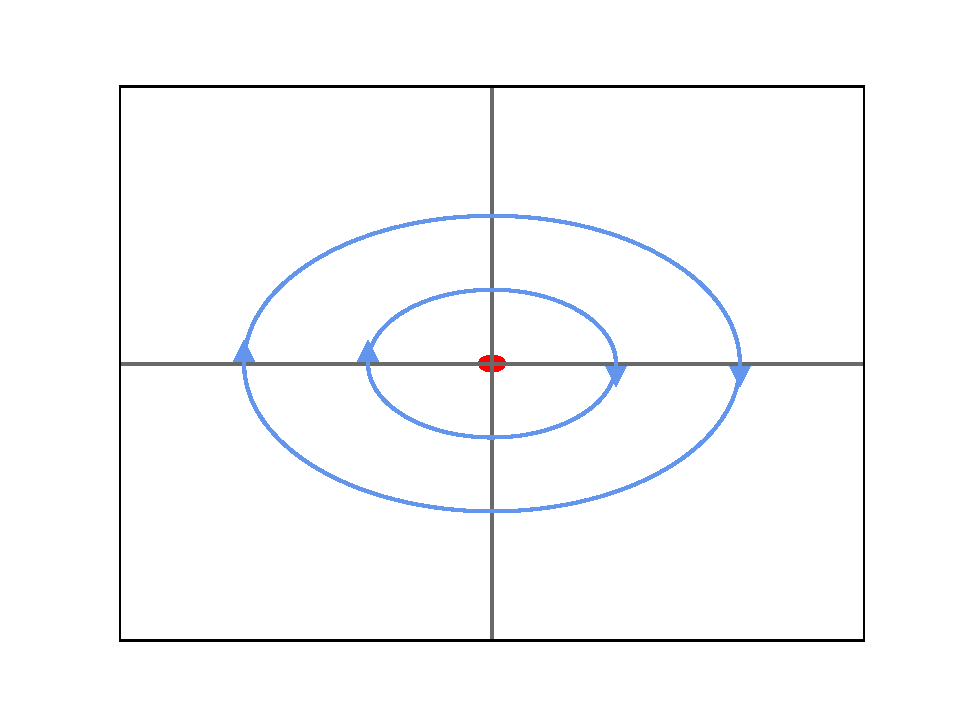
\includegraphics[scale=0.4]{hyperbolic.pdf}}
	\subfigure{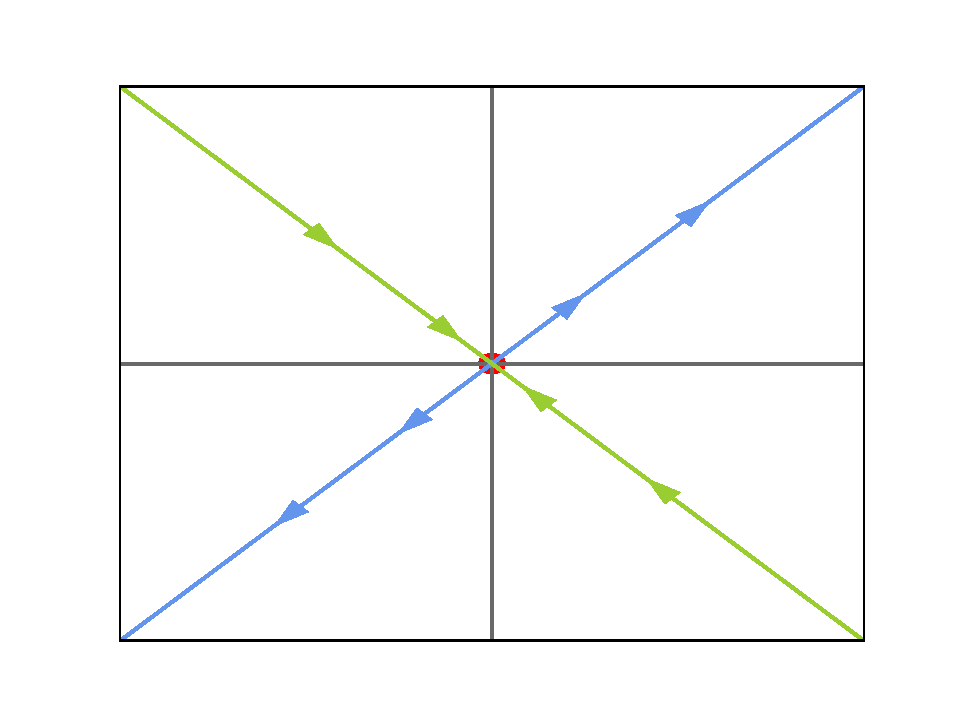
\includegraphics[scale=0.4]{hyperbolic2.pdf}}
	\caption{Punto fijo elíptico (izquierda) e hiperbólico (derecha) en el espacio fase.}
	\label{hiperbolic}
\end{figure}


En el caso hiperbólico existen dos comportamientos que nos interesan, marcados con las líneas azul y verde de la figura \ref{hiperbolic}, tales corresponden a los eigenespacios asociados a los vectores propios de $\mathbf{A}$. Existe un teorema importante de Hart\-man-Grob\-man que asegura que hay una vecindad del punto fijo hiperbólico tal que el mapeo es topológicamente conjugado a su linealización \cite{Meiss,Meyer,Juergen}. Dicho de otra manera, hay vecindades $U$ de $\mathbf{x}_{*}$, $V$ de $0 \in \mathbf{R}^{2}$ y un homeomorfismo $h:U\rightarrow V$ tal que $h$ mapea trayectorias de $\mathbf{f}$ en trayectorias del sistema lineal. De esta manera se justifica trabajar con un sistema lineal.



\section{Conjuntos invariantes}
Alrededor de un punto fijo existen ciertos conjuntos que expresan algunas ca\-rac\-te\-rís\-ti\-cas del sistema; estos conjuntos tienen que ver directamente con lo que se observa en la figura \ref{hiperbolic}. Para entender su comportamiento, se usa la definición de un conjunto invariante.

\begin{defini}[\textit{\textsc{Conjunto invariante}}\cite{Ott}]
\textit{Un conjunto invariante es un subconjunto $\mathbf{I} \subset \mathbf{E}$ del espacio fase tal que para cualquier $\mathbf{x}_{i}\in  \mathbf{I}$  y $ n\in\mathbb{N}$ \\
\begin{center}
$\mathbf{f}^{n}(\mathbf{x}_{i}) \in \mathbf{I}$.
\end{center}
}
\end{defini}
Es decir que cualquier elemento tomado en el conjunto se queda en el conjunto bajo la aplicación del mapeo. \\

Lo siguiente se enfoca en el estudio de conjuntos invariantes asociados a puntos fijos hiperbólicos. Si $\mathbf{x}_{*}$ es un punto fijo hiperbólico entonces se define las \textit{variedades estable} e \textit{inestable} como
\begin{eqnarray}
W^{s}=\lbrace \mathbf{x} : \mathbf{f}^{n}(\mathbf{x})\rightarrow \mathbf{x}_{*} \quad \mathrm{cuando} \quad n\rightarrow \infty \rbrace
\label{variedad estable}
\end{eqnarray}

\begin{eqnarray}
W^{u}=\lbrace \mathbf{x} : \mathbf{f}^{n}(\mathbf{x})\rightarrow \mathbf{x}_{*} \quad \mathrm{cuando} \quad n\rightarrow -\infty \rbrace.
\label{variedad inestable}
\end{eqnarray}


Localmente las variedades resultan ser tangentes a los subespacios generados por los vectores propios

\begin{eqnarray*}
\lbrace \beta \pmb v_{1} : \beta\in \mathbb{R} \rbrace,
\end{eqnarray*}

\begin{eqnarray*}
\lbrace \alpha \pmb v_{2} : \alpha\in \mathbb{R}\rbrace.
\end{eqnarray*}
Esto se resume en el siguiente teorema.







\begin{thm}[\underline{\textit{De la variedad estable}} \cite{Mateo}]
\textit{Sea un sistema de la forma $\mathbf{x}_{n+1}=\mathbf{f}(\mathbf{x}_{n})$ con un punto fijo hiperbólico en el origen. Sean $E^{s}$ y $E^{u}$ los subespacios estables e inestables de la linealización del sistema,
 $\mathbf{y}_{n+1}=\mathbf{J}\mathbf{y}_{n}$ donde $\mathbb{J}$ es la matriz Jacobiana en el origen . Si 
 $\mid \mathbf{y_{n+1}}-\mathbf{J}\mathbf{y_{n}}\mid = O(\mathbf{y}_{n}^{2})$
 entonces existen localmente variedades estables e inestables con las mismas dimensiones que $E^{s}$,$E^{u}$ y que son tangentes a éstos en cero respectivamente, dadas por}
\begin{eqnarray*}
W^{s}_{\mathrm{loc}}(\mathbf{x}_{*})= \lbrace \mathbf{x}_{*} : \mathbf{f}^{k}(\mathbf{x}_{n})\rightarrow \mathbf{x}_{*} \quad\mathrm{cuando}\quad k \rightarrow \infty \rbrace,
\end{eqnarray*}
\begin{eqnarray*}
W^{u}_{\mathrm{loc}}(\mathbf{x}_{*}) = \lbrace \mathbf{x}_{*} : \mathbf{f}^{k}(\mathbf{x}_{n})\rightarrow \mathbf{x}_{*} \quad\mathrm{cuando}\quad k \rightarrow -\infty \rbrace.
\end{eqnarray*}
\end{thm}

Es necesario mencionar que una variedad estable no puede cruzarse con otra variedad estable, lo mismo sucede con las inestables, así como con la intersección de una variedad consigo misma. Para entender esto suponga que se tienen dos puntos fijos diferentes con sus respectivas variedades inestables asociadas. Suponga que las variedades se cruzan en algún punto. Si esto pasará, la órbita hacia atrás de cualquiera de los dos puntos empezando en la intersección debería aproximarse a ambos puntos fijos, lo cual es imposible pues son diferentes. El argumento para la intersección de las estables es similar. Lo que sí puede suceder es la intersección de una variedad estable con una inestable, asociadas al mismo punto fijo; a esto se le llama una \textit{intersección homoclínica}. Si la intersección es entre variedades asociadas a diferentes puntos fijos entonces se llama \textit{heteroclínica} \cite{Ott}. Resulta además que si dos variedades, estable e inestable, se cortan en un punto se cortarán una infinidad de veces más. \\


El cálculo de variedades alrededor de un punto fijo es un problema difícil de atacar analíticamente, pues su comportamiento puede ser muy complejo; por ello es necesario explotar al máximo la linealización que se hace del sistema, para poder, con métodos numéricos o semianalíticos, calcular las variedades. 




\section{Sistemas Hamiltonianos}
Los sistemas Hamiltonianos son una clase particular de los sistemas dinámicos. En 1834 William R. Hamilton reformuló la ecuación de Newton ($\mathbf{F}=m\mathbf{a}$) para un conjunto de partículas puntuales en un campo de fuerzas. Cuando la fuerza $\mathbf{F}$ es conservativa es posible escribir a la fuerza como  el negativo del gradiente de una función potencial:
\begin{eqnarray}
\mathbf{F}=-\nabla V. \label{fuerza potencial}
\end{eqnarray}
La ecuación \eqref{fuerza potencial} se puede convertir en un sistemas de ecuaciones diferenciales, con $\mathbf{x} \in \mathbb{R}^{n}$
\begin{eqnarray}
\frac{d\mathbf{x}}{dt}=\mathbf{v},
\label{fuerza sistema dif a}
\end{eqnarray}
\begin{eqnarray}
m\frac{d\mathbf{v}}{dt}=-\nabla V.
\label{fuerza sistema dif b}
\end{eqnarray}
En términos de coordenadas generalizadas, las ecuaciones \ref{fuerza sistema dif a},\ref{fuerza sistema dif b} pueden obtenerse a partir de una función muy particular llamada Hamiltoniana \ref{Hamiltoniano-general}. En la Hamiltoniana $p$ denota el momento, $q$ la posición, $V(q)$ una función potencial y se ha tomado m=1.
\begin{eqnarray}
H(p,q)=\frac{p^{2}}{2}+V(q),
\label{Hamiltoniano-general}
\end{eqnarray}
las ecuaciones de movimiento que se obtienen de \ref{Hamiltoniano-general} son:
\begin{eqnarray}
\frac{dq}{dt}=\frac{\partial H}{\partial p},
\label{1ec de mov}
\end{eqnarray}
\begin{eqnarray}
\frac{dp}{dt}=-\frac{\partial H}{\partial q}.
\label{2ec de mov}
\end{eqnarray}

Para un sistema en el que el potencial se aplica de manera discreta, en pasos de tiempo $t_{n}$ con $n\in\mathbb{Z}$ y $t\in\mathbb{R}$, en periodos de tiempo $T$, la Hamiltoniana es:
\begin{eqnarray}
H(q,p)=\frac{p^{2}}{2}+V(q)\sum_{n=-\infty}^{\infty}\delta(t-nT).
\label{ec de hamilton} 
\end{eqnarray}
Análogas a las ecuaciones \ref{1ec de mov},\ref{2ec de mov}, pero usando \ref{ec de hamilton} se tiene 
\begin{eqnarray}
\frac{dq}{dt}=p\quad
\label{SistemaH1}
\end{eqnarray}
\begin{eqnarray}
\frac{dp}{dt}=-\frac{dV(q)}{dq}\sum_{n=-\infty}^{\infty}\delta(t-nT).
\label{SistemaH2}
\end{eqnarray}
Al tomar $T=1$, sin pérdida de generalidad, e integrar la ecuación \eqref{SistemaH1} en el intervalo $[t_{n}-\epsilon,t_{n+1}-\epsilon]$ con $\epsilon>0$
\begin{eqnarray}
\int_{t_{n}-\epsilon}^{t_{n+1}-\epsilon}\frac{dq}{dt}dt=\int_{t_{n}-\epsilon}^{t_{n+1}-\epsilon}pdt.
\label{integral1}
\end{eqnarray}
usando el teorema fundamental del cálculo, se obtiene
\begin{eqnarray}
q(t_{n+1}-\epsilon)-q(t_{n}-\epsilon)=\epsilon p(t_{n}-\epsilon)+(1-\epsilon)p(t_{n+1}-\epsilon).
\label{integral2}
\end{eqnarray}
Haciendo lo mismo para la ecuación \eqref{SistemaH2}
\begin{eqnarray}
\int_{t_{n}-\epsilon}^{t_{n+1}-\epsilon}\frac{dp}{dt}dt=\int_{t_{n}-\epsilon}^{t_{n+1}-\epsilon}-\frac{dV(q)}{dq}\sum_{n=-\infty}^{\infty}\delta(t-n),
\label{integral3}
\end{eqnarray}
resulta
\begin{eqnarray}
p(t_{n+1}-\epsilon)-p(t_{n}-\epsilon)=-\frac{dV(q)}{dq}.
\label{integral4}
\end{eqnarray}
Tomando el límite cuando $\epsilon\rightarrow 0$ en las ecuaciones \eqref{integral2}\eqref{integral4} se obtiene
\begin{eqnarray}
q_{n+1}=p_{n+1}+q_{n},
\label{sistema hamilton a}
\end{eqnarray}
\begin{eqnarray}
p_{n+1}=p_{n}-\frac{dV(q_{n})}{dt}.
\label{sistema hamilton b}
\end{eqnarray}






Las ecuaciones \eqref{sistema hamilton a},\eqref{sistema hamilton b} ya está en forma de un sistema de los que se estudió anteriormente. Para linealizar el sistema se calcula el jacobiano
\begin{eqnarray}
\mathbf{J}=\frac{\partial(q_{n+1},p_{n+1})}{\partial(q_{n},p_{n})},
\end{eqnarray}
con $q_{n+1}=q(t_{n+1})$ y análogamente para $p$. Es justo de este sistema linealizado de donde se obtiene información a partir de aplicar los teoremas y resultados de las secciones anteriores. 










\section{Método de parametrización}
Como ya se observó en la sección anterior, encontrar las variedades asociadas a un punto fijo no es trivial. Los métodos analíticos se vuelven no sólo tediosos si no que hacen necesario que el análisis de un sistema se haga de forma particular. Y para encontrar tales variedades hay que explotar los conocimientos que se tienen sobre los sistemas. Algunas de estas características son realmente simples, por ejemplo se sabe que en un punto hiperbólico resultarán dos variedades asociadas a los valores propios de la matriz que representa el sistema linealizado. Este trabajo se concentra en los sistemas Hamiltonianos; ya que estos preservan el área y son importantes en la física; sin embargo el método funciona también para sistemas no Hamiltonianos. Esta sección tiene como objetivo describir el método de parametrización desarrollado por X. Cabré, E. Fontich y R. de la Llave \cite{Haro}. El método fue desarrollado de manera general para conjuntos invariantes, estables e inestables, en puntos hiperbólicos, tratándose de un método semianalítico, es decir parte computacional y parte analítica.\\

%A David no le gusto esto:
%Para ahondar en el método recordemos que anteriormente mencionamos que los conjuntos \eqref{variedad estable}, \eqref{variedad inestable} son conjuntos invariantes. Por otro lado también recordemos la definición de sistema dinámico que nos dice que se trata de un semigrupo actuando sobre un espacio $M$, la manera en la que se genera el sistema es con un difeomorfismo 


Recuerde, que anteriormente se menciona que los conjuntos \eqref{variedad estable}, \eqref{variedad inestable} son conjuntos invariantes; además la definición de sistema dinámico dice que se trata de un mapeo iterado $\mathbf{f}:M \rightarrow M$. Considerando esto, en el espacio $M$ se define una inmersión inyectiva $\mathcal{P}:\Theta \rightarrow M$ con $\Theta\subset \mathbb{R}$, siendo esto una parametrización de la variedad $W$ en términos de variables locales $\theta \in \Theta$. La variedad invariante parametrizada por $\mathcal{P}$ junto con $g:\Theta \rightarrow \Theta$, deben cumplir 
\begin{eqnarray}
\mathbf{f} \circ \mathcal{P} =\mathcal{P}  \circ g,  \label{Ecua de invariancia}
\end{eqnarray}
llamada ecuación de invariancia \cite{Haro}.
Es decir $\mathcal{P}$ y $g$ son de tal forma que hacen que el siguiente diagrama conmute
\begin{eqnarray}
\xymatrix{
\Theta\subset\mathbb{R} \ar[d]^{\mathcal{P}} \ar[r]^{g} & \Theta\subset\mathbb{R} \ar[d]^{\mathcal{P}} \\
M\subset\mathbb{R}^{n} \ar[r]^{\mathbf{f}} & M\subset\mathbb{R}^{n}
}\label{conmutativo}
\end{eqnarray}

\begin{figure}[h!]
	\centering
	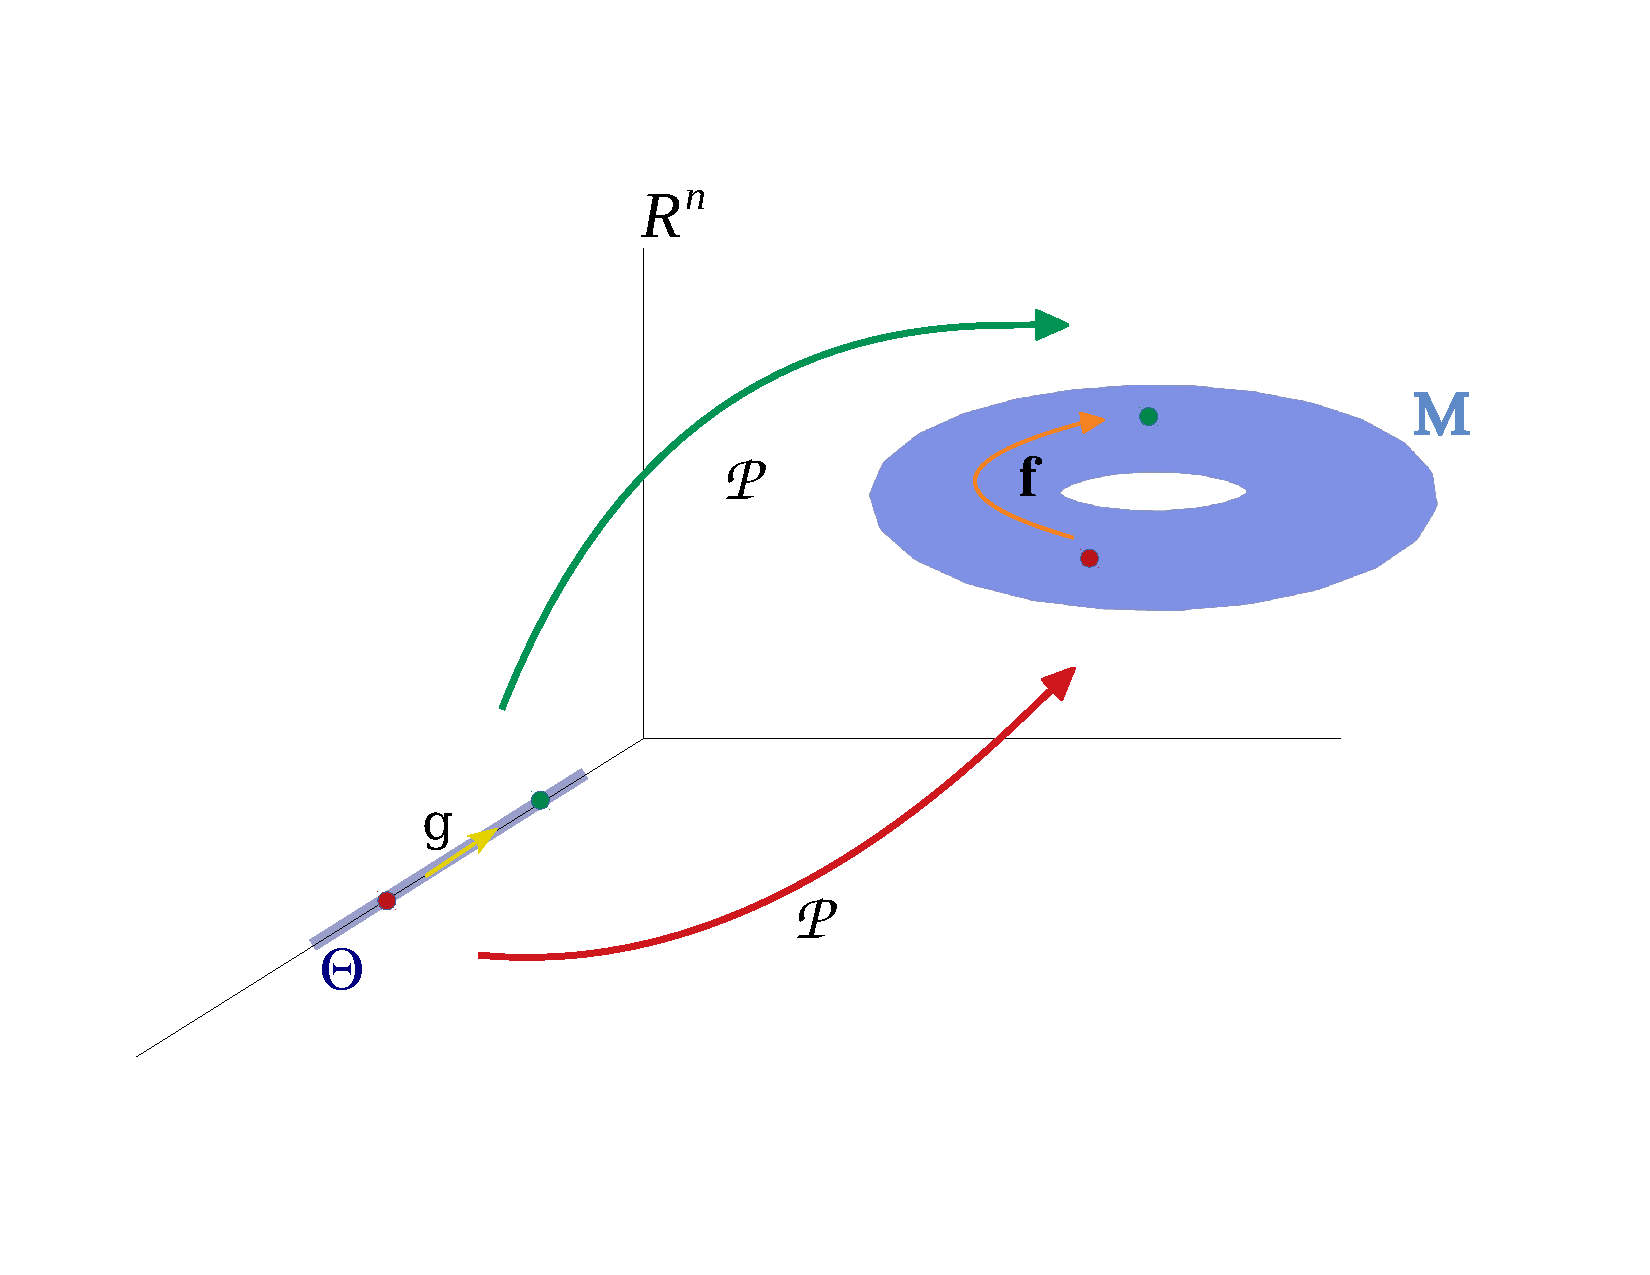
\includegraphics[scale=0.4]{diagrama-conmutativo}
	\caption{Representación grafica del diagrama \eqref{conmutativo}.}
	\label{diagrama-conmutativo}
\end{figure}


En este sentido $g$ representa un subsistema de $\mathbf{f}$, en otras palabras $g$ contiene la dinámica del mapeo pero sobre $\Theta$. El objetivo del método de parametrización es encontrar $\mathcal{P}$ y $g$ que cumplan la ecuación de invariancia \eqref{Ecua de invariancia}. Aunque no se conozca la dinámica interna de $g$, es fácil ver que $\mathcal{P}$ y $g$ son soluciones de \eqref{Ecua de invariancia}; al observar el diagrama \eqref{conmutativo} es claro que la composición también es solución y eso proporciona una libertad para resolver la ecuación. El obstáculo, no conocer $g$, se puede pasar si se escoge una forma de parametrización que dependa del sistema; en el método de parametrización se tienen descritas dos formas: la forma gráfica y la forma normal. De aquí en adelante se usa el método de la forma gráfica, que es la forma más simple de parametrización. Consiste en adaptar la forma de la parametrización $\mathcal{P}$ a la forma de las variedades, la cual está relacionada con la dirección que proporcionan los vectores propios. Para el caso de una matriz hiperbólica de $2\times 2$ sus vectores propios indican, suficientemente cerca del punto fijo, la dirección de cada variedad. \\


La forma en la que se escoge $g$, en la mayoría de las veces, es polinomial de tal manera que se adapte a la forma del mapeo. Sin embargo la elección puede ser diferente dependiendo del sistema. Se escogió la dependencia más sencilla para las variables del mapeo $\mathbf{f}(x,y)$ \eqref{fun g}, en la que se incluye el valor propio del sistema $\lambda$; para el caso hiperbólico es suficientes con esto
\begin{eqnarray}
g(t) = \lambda t.
\label{fun g}
\end{eqnarray}
Obteniendo del lado derecho de la ecuación \eqref{Ecua de invariancia} un polinomio. \\

Al conocer las variedades parametrizadas; es importante tener una función que indique qué tan acertada es la parametrización. La primera y más fácil forma de calcular el error es a partir de la ecuación \eqref{Ecua de invariancia}, mediante la norma de la resta
\begin{eqnarray}
E_{n}(t) = \parallel \mathbf{f} \circ \mathcal{P}_{n}(t) - \mathcal{P}_{n} \circ g(t) \parallel_{\infty}.  \label{Ecua de invariancia resta}
\end{eqnarray}
Este error será el asociado a la variación con respecto a la ecuación de invariancia. El subíndice $n$ denota el orden de la parametrización. Dado que depende del parámetro, se espera que el error vaya creciendo conforme se evalúa en valores de $t$ más alejados del punto fijo. Otra forma de evaluar qué tan lejos se puede llegar con la parametrización es ver el comportamiento de los coeficientes de los polinomios asociados. Al tener los polinomios que parametrizan la variedad, con coeficientes $a_{n}$ y $b_{n}$ de orden $n$, es posible evaluar el cociente entre ellos
\begin{eqnarray}
\lim_{n\rightarrow\infty}\frac{a_{n}}{a_{n+1}},\label{hadamard}
\end{eqnarray} 
con $(a_{0},b_{0})=\mathbf{x}_{*}$ los coeficientes de orden cero. Lo que se hace con este cociente es estudiar la convergencia según Hadamard \citep{lang}. Si el límite anterior tiende a cero entonces la serie $a_{n}$ converge. Otra forma de evaluarlo es usando la relación de tres términos \citep{Chang}.
\begin{eqnarray}
\lim_{i\rightarrow\infty} \left[ i\left(\frac{a_{i+1}}{a_{i}}\right)-(i-1)\left(\frac{a_{i}}{a_{i-1}}\right) \right].
\label{tres terminos}
\end{eqnarray}
Aunque el método se aplica de la misma manera para los puntos fijos de mapeos de dos dimensiones, la parametrización será diferente en cada mapeo y en cada punto fijo, por lo que la convergencia de cada parametrización es distinta. 
